\documentclass[10pt,usenames,dvipsnames]{beamer}
\usepackage{pgfpages}
%\setbeameroption{show notes on second screen}

\usepackage{xcolor}

\usetheme[progressbar=foot, numbering=counter, titleformat title=smallcaps, titleformat frame=smallcaps, sectionpage=progressbar, subsectionpage=progressbar]{metropolis}
\usepackage{appendixnumberbeamer}

\usepackage{booktabs}
\usepackage[scale=2]{ccicons}

\usepackage{pgfplots}
\usepgfplotslibrary{dateplot}

\usepackage{xspace}
\newcommand{\themename}{\textbf{\textsc{metropolis}}\xspace}

\usepackage{minted}
\usepackage{verbatim}
\usepackage{graphicx}
\usepackage{subcaption}
\usepackage{setspace}
\usepackage{listings}
\usepackage{appendixnumberbeamer}

\setsansfont[BoldFont={Fira Sans SemiBold}]{Fira Sans Book}
\usebackgroundtemplate{
\includegraphics[width=\paperwidth,height=\paperheight]{imgs/background2.png}}


% custom colors
\definecolor{progress-bar-fg}{HTML}{C57502}
\definecolor{progress-bar-bg}{HTML}{FFFFFF}%gray : BABABA
\definecolor{minted-bg}{HTML}{B9DCE2}
\definecolor{keyword-green}{HTML}{007F00}
\setbeamercolor{progress bar}{fg=progress-bar-fg, bg=progress-bar-bg}
\setbeamercolor{title}{bg=, fg=white}
\setbeamercolor{section title}{bg=, fg=white}
\setbeamercolor{frametitle}{bg=, fg=white}
\setbeamercolor{normal text}{bg=, fg=black}

% custom fonts
\setbeamercolor{page number in head/foot}{fg=green}
\setbeamerfont{page number in head/foot}{size=\normalsize}

% line stretch
\renewcommand{\baselinestretch}{1.5}

\AtBeginEnvironment{minted}{
  \renewcommand{\fcolorbox}[4][]{#4}
  \renewcommand{\baselinestretch}{1.0}
  \fontsize{9}{9}\selectfont
}

% listings config

\lstset{
    showstringspaces=false,
    basicstyle=\ttfamily,
    keywordstyle=\color{blue},
    commentstyle=\color[grey]{0.6},
    stringstyle=\color[RGB]{255,150,75}
}


\lstdefinelanguage{kotlin}{
  keywords={package, as, typealias, this, super, val, var, fun, for, null, true, false, is, in, 
throw, return, break, continue, object, if, try, else, while, do, when, yield, typeof, yield, 
typeof, class, interface, enum, object, override, public, private, get, set, import, abstract, field, },
  keywordstyle=\color{keyword-green}\bfseries,
  ndkeywords={@Deprecated, Iterable, Int, Integer, Float, Double, String, Runnable, dynamic},
  ndkeywordstyle=\color{BurntOrange}\bfseries,
  emph={println, return@, forEach,},
  emphstyle={\color{OrangeRed}},
  identifierstyle=\color{black},
  sensitive=true,
  commentstyle=\color{gray}\ttfamily,
  comment=[l]{//},
  morecomment=[s]{/*}{*/},
  stringstyle=\color{ForestGreen}\ttfamily,
  morestring=[b]",
  morestring=[s]{"""*}{*"""},
}

\newcommand{\inlinecode}[2]{\colorbox{minted-bg}{\lstinline[language=#1]$#2$}}

\newcommand{\scalainline}[1]{\inlinecode{scala}{#1}}
\newcommand{\ktinline}[1]{\inlinecode{kotlin}{#1}}

\begin{comment}
 binary op --> big change (no details)
 super calls
 properties + interfaces
 lambdas
 Kotlin js()
 
 if time permits
 - enum
 - safety operators
 - null safety 
 
 + have a hello world project ready just in case
 
 
 Comments for presentation
 - page number in white and bigger
 - background -> need more contrast between text and background
 - s. 10 -> inverse the two : kotlin example first, avoid explaining with text what code can show
 - s. 15 -> applystatic first, applystatically ~= invokespecial in JVM calls an instance method with static dispatch
\end{comment}


% title slide
\title{Production Level Tooling for the Kotlin to Scala.js Compiler}
\subtitle{Master Semester Project}
\date{}
\author{Florian Alonso}
\institute{EPFL - Programming Methods Laboratory (LAMP) }
%\titlegraphic{\hfill
\includegraphics[height=1.0cm]{imgs/epfl_logo.png}}

\begin{document}

\begin{frame}
  \titlepage
\end{frame}

\begin{frame}[fragile]{Contents}
  \setbeamertemplate{section in toc}[sections numbered]
  \tableofcontents[hideallsubsections]
\end{frame}

\section{Introduction}

\begin{frame}{Project Goals}
 \begin{itemize}
  \item Continue the work started by Guillaume Tournigand and Lionel Fleury
  \item Validate the generic nature of the Scala.js IR
  \item Compile Kotlin Standard Library to the Scala.js IR
  \item Develop Gradle tooling
 \end{itemize}

\end{frame}
\begin{comment}
\begin{frame}[fragile]{Kotlin}
  \begin{itemize}
   \item Targetting multiple platforms
    \begin{itemize}
     \item JVM
     \item Android 
     \item The browser (JavaScript)
    \end{itemize}
   \item Null safety
   \item Large standard library
  \end{itemize}
\end{frame}

\begin{frame}[fragile]{Hello Kotlin}

  \begin{minted}[bgcolor=minted-bg]{kotlin}
class Greater {
  fun great(s: String) {
    println("Hello $s")
  }
}

fun main(args: Array<String>) {
  val name = "Kotlin"
  val g = Greater()
  g.great(name) // prints "Hello Kotlin"
}
  \end{minted}

\end{frame}

% --> move to benchmarks
\begin{frame}{Scala.js}
 \begin{itemize}
  \item Scala compiled to JavaScript
  \item Optimizations
    \begin{itemize}
     \item Dead-code elimination
     \item Inlining
     \item Constant-folding
     \item Closure eliminations
     \item ...
    \end{itemize}
  \item Makes use of Google Closure Compiler

 \end{itemize}

\end{frame}

\end{comment}


\section{Main improvements}

%%%%%%%%%%%%%%%%%%%%%%%%%%%%%% BINARY AND UNARY %%%%%%%%%%%%%%%%%%%%%%%%%%%%%%

\subsection{Binary and unary operations}


\begin{frame}[fragile]{Binary and unary operations}
  Endured an important refactoring because of Scala.js internal changes.
  
  \begin{itemize}
   \item Each IR type has its own representation
   \item Appropriate conversions were needed
  \end{itemize}
  
  The resulting logic is closer to what is done in Scala.js itself.

\end{frame}

%%%%%%%%%%%%%%%%%%%%%%%%%%%%%% NULL SAFETY %%%%%%%%%%%%%%%%%%%%%%%%%%%%%%
\subsection{Null safety operators}


\begin{frame}[fragile]{Null safety operators}
 Kotlin provides its own way of avoiding (or dealing with) NullPointerExceptions :
 
 \begin{itemize}
  \item Safe calls with \ktinline{?.}
  \item Default values with the elvis operator \ktinline{?:}
  \item Not-null assertions with \ktinline{!!}
 \end{itemize}

 These operators are translated as conditional expressions. Expressions to be tested are first assigned to temporary variables.
 
\end{frame}

\begin{frame}[fragile]{Null safety operators - Safe call and elvis operator}

\onslide<1->
\begin{minted}[bgcolor=minted-bg]{kotlin}
fun nullSafety(canBeNull: String?): Int {
    return canBeNull?.length ?: 0
}
\end{minted}

\onslide<2->
 \begin{minted}[bgcolor=minted-bg]{scala}
static def nullSafety__T__I(canBeNull: T): int = {
  val tmp$1: T = canBeNull;
  if ((tmp$1 !== null)) {
    tmp$1.length__I()
  } else {
    null
  }
}
 \end{minted}

\end{frame}

\begin{frame}[fragile]{Null safety operators - Safe call and elvis operator}
\begin{minted}[bgcolor=minted-bg]{kotlin}
fun nullSafety(canBeNull: String?): Int {
    return canBeNull?.length ?: 0
}
\end{minted}

 \begin{minted}[bgcolor=minted-bg, highlightlines={4-9}]{scala}
static def nullSafety__T__I(canBeNull: T): int = {
  return {
    val tmp$0: jl_Integer = {
      val tmp$1: T = canBeNull;
      if ((tmp$1 !== null)) {
        tmp$1.length__I()
      } else {
        null
      }
    };
    if ((tmp$0 !== null)) {
      tmp$0.asInstanceOf[I]
    } else {
      0
    }
  }
}
 \end{minted}

\end{frame}

\begin{frame}[fragile]{Null safety operators - Not-null assertion}

\begin{minted}[bgcolor=minted-bg]{kotlin}
fun assertNotNull(cantBeNull: Any?): Unit {
    cantBeNull!!
}
\end{minted}

\onslide<2->
 \begin{minted}[bgcolor=minted-bg]{scala}
static def assertNotNull__O__V(cantBeNull: any) {
  val tmp$0: any = cantBeNull;
  if ((tmp$0 !== null)) {
    tmp$0
  } else {
    throw new jl_NullPointerException().init___()
  }
}
 \end{minted}
\end{frame}


%%%%%%%%%%%%%%%%%%%%%%%%%%%%%% ACCESSORS %%%%%%%%%%%%%%%%%%%%%%%%%%%%%%

\subsection{Properties accessors}


\begin{frame}{Properties accessors}
  In Kotlin, properties can either make use of default accessors or define custom ones.
  
  When a property makes use of a default accessor or uses the \ktinline{field} keyword, a backing field is generated.

\end{frame}

\begin{frame}[fragile]{Properties accessors - Backing field in Scala}

  The \ktinline{field} keyword is simply a placeholder for the compiler-generated backing field.
  
  \begin{minted}[bgcolor=minted-bg]{kotlin}
class Accessors {
  var counter = 0
    get() = field
    set(value: Int) { field = value }
}
  \end{minted}
  
  \onslide<2->
  In Scala, a backing field would look like this : 
  
  \onslide<2->
  \begin{minted}[bgcolor=minted-bg]{scala}
class Accessors {
  private var _counter = 0 // <- the backing field
  def counter = _counter
  def counter_= (value: Int) = { _counter = value }
}
  \end{minted}

\end{frame}

\begin{frame}[fragile]{Properties accessors - Kotlin example}

\onslide<1->
  \begin{minted}[bgcolor=minted-bg]{kotlin}
class Accessors {
  var counter = 0 // with backing field

  val msg // without backing field
    get() = "Hello Kotlin"
}
  \end{minted}
\onslide<2->
  \begin{minted}[bgcolor=minted-bg]{scala}
class LAccessors extends O {
  var counter: int
  def counter__I(): int = { this.counter }
  def counter__I__V(set: int) {
    this.counter = set
  }
  def msg__T(): T = {
    ("" +[string] "Hello Kotlin")
  }
  def init___() {
    this.O::init___();
    this.counter = 0
  }
}
  \end{minted}
\end{frame}

%%%%%%%%%%%%%%%%%%%%%%%%%%%%%% INTERFACES %%%%%%%%%%%%%%%%%%%%%%%%%%%%%%

\subsection{Interfaces}

\begin{comment}
 \begin{itemize}
  \item Interfaces are translated with abstract method bodies
  \item They can also define default implementations for their methods :
    \begin{itemize}
     \item These are represented as static definitions inside a separate class
     \item They all take an instance of the implementing class as first parameter
     \item If not overridden, bridges are generated in implementing classes
    \end{itemize}
 \end{itemize}
\end{comment}

\begin{frame}{Interfaces}
  \begin{itemize}
   \item Interfaces are translated with abstract method bodies
   \item The default implementations are stored in a separate class
  \end{itemize}

\end{frame}

\begin{frame}[fragile]{Interfaces - A default implementation}
 \onslide<1->
 \begin{minted}[bgcolor=minted-bg]{kotlin}
interface Dummy {
  val a: String // no backing field allowed !
    get() = "Hello from an interface"
}
 \end{minted}
 
 \onslide<2->
 \begin{minted}[bgcolor=minted-bg]{scala}
interface LDummy {
  def a__T(): T = <abstract>
}

class LDummy$DefaultImpls extends O {
  static def a__LDummy__T($this: LDummy): T = {
    ("" +[string] "Hello from an interface")
  }
}
 \end{minted}


\end{frame}


\begin{frame}[fragile]{Interfaces - Bridge generation}

 \onslide<1->
 \begin{minted}[bgcolor=minted-bg]{kotlin}
interface Dummy {
  val a: String
    get() = "Hello from an interface"
}

class MyClass: Dummy
 \end{minted}
 
 \onslide<2->
 \begin{minted}[bgcolor=minted-bg]{scala}

class LMyClass extends O implements LDummy {
  def a__T(): T = {
    LDummy$DefaultImpls::a__LDummy__T(this)
  }
  // init
}
 \end{minted}
 
\end{frame}

%%%%%%%%%%%%%%%%%%%%%%%%%%%%%% SUPER CALLS %%%%%%%%%%%%%%%%%%%%%%%%%%%%%%

\subsection{Super calls}

\begin{frame}{Super calls}
 \only<1> {
 Super calls must also be translated depending on which instance they refer to :
 
 \begin{itemize}
  \item Reference to a (parent) class
  \item Reference to an interface's default implementation
 \end{itemize}
 }
 
 \only<2>{
  Interface :
  \begin{itemize}
   \item \scalainline{ApplyStatic()} applies a static method for a given class type.
  \end{itemize}
  
  Parent class :
  \begin{itemize}
   \item \scalainline{ApplyStatically()} indicates a static dispatch to a given class type on the receiver's instance (\~= invokespecial).
  \end{itemize}

 }
\end{frame}

\begin{frame}[fragile]{Super calls - Example}
 \begin{minted}[bgcolor=minted-bg]{kotlin}
interface I {
  val a: String
    get() = "Hello from parent interface"
}

open class MyParent {
  open val a: String = "Hello from parent class"
}

class MyChild: MyParent(), I {
  override val a: String = "Hello from child"

  fun example() {
    super<I>.a
    super<MyParent>.a
    this.a
  }
}
 \end{minted}

\end{frame}

\begin{frame}[fragile]{Super calls - Example}
\begin{comment}
 
  val a$1: T
  def a__T(): T = {
    this.a$1
  }
  
  
  def init___() {
    this.LMyParent::init___();
    this.a$1 = ("" +[string] "Hello from child")
  }
\end{comment}

 \begin{minted}[bgcolor=minted-bg, highlightlines={5-6}]{scala}
class LMyChild extends LMyParent implements LI {
  // 'a' field accessors
  
  def example__V() {
    LI$DefaultImpls::a__LI__T(this); // ApplyStatic
    this.LMyParent::a__T(); // ApplyStatically
    this.a__T();
    (void 0)
  }
  
  // init call
}
 \end{minted}

\end{frame}

%%%%%%%%%%%%%%%%%%%%%%%%%%%%%% LAMBDA EXPRESSIONS %%%%%%%%%%%%%%%%%%%%%%%%%%%%%%

\subsection{Lambdas}

\begin{frame}[fragile]{Lambdas} 
 In Kotlin JS, Kotlin.FunctionX are JavaScript functions.
 
 In Scala.js, Scala functions are wrapped. They are JavaScript objects.
 
 % sjs_AnonFun = wrapper to provide scala function interface --> semantics of the language
 % In Kotlin FunctionX is a js functions
 
 To stick to the Kotlin JS semantics, translate them as closures :
 \begin{itemize}
  \item Formal parameters of type \ktinline{Any}
  \item Inside the body, parameters are cast to the declared type
 \end{itemize}
\end{frame}

\begin{frame}[fragile]{Lambdas - Example}
 \onslide<1->
 \begin{minted}[bgcolor=minted-bg]{kotlin}
class Dummy {
  var times: (Int, Int) -> Int = { a,b ->
    a * b
  }
}
 \end{minted}
 \onslide<2->
 \begin{minted}[bgcolor=minted-bg]{scala}
// Inside the init call of a class
this.times = (lambda<$this: LDummy = this>(
  closureargs$a: any,  closureargs$b: any) = {
  val a: int = closureargs$a.asInstanceOf[I];
  val b: int = closureargs$b.asInstanceOf[I];
  (a *[int] b)
})
 \end{minted}
 
\end{frame}
 
%%%%%%%%%%%%%%%%%%%%%%%%%%%%%% Kotlin JS Function %%%%%%%%%%%%%%%%%%%%%%%%%%%%%%

\subsection{Kotlin \ktinline{js} function}

\begin{frame}[fragile]{Kotlin \ktinline{js} function}
  Allows to write pure JavaScript inside Kotlin code:
  
  \begin{minted}[bgcolor=minted-bg]{kotlin}
js("Kotlin.identityHashCode")(3)
  \end{minted}

%  Because the Scala.js IR doesn’t allow inserting a JS string verbatim inside the code. This is to prevent breaking IR abstractions.

  Breaks the compiler abstraction. The Scala.js IR doesn't allow that.
  
  It must therefore be handled case by case.

\end{frame}

%%%%%%%%%%%%%%%%%%%%%%%%%%%%%% OTHER ADDITIONS %%%%%%%%%%%%%%%%%%%%%%%%%%%%%%
\subsection{Other additions}

\begin{frame}{Other additions}
 \begin{itemize}
  \item Qualified this
  \item Type checks and casts
  \item Enum classes
  \item Anonymous objects
 \end{itemize}

\end{frame}


\section{Gradle Plugin}

\begin{frame}{Plugin overview}
 \begin{itemize}
  \item Pass the Kotlin source files to the compiler
  \item Output the SJSIR files
  \item Use the Scala.js linker to produce a JS file
  \item Success !
 \end{itemize}

\end{frame}


\begin{frame}[fragile]{Plugin setup - build.gradle}
\begin{minted}[bgcolor=minted-bg, breaklines=true, highlightlines={12}]{kotlin}
buildscript {
  ext.kotlin_version = "1.1.61"
    
  repositories { mavenCentral(); mavenLocal() }

  dependencies {
    classpath "org.jetbrains.kotlin:kotlin-gradle-plugin:$kotlin_version"
    classpath "ch.epfl.k2sjs:kotlin2sjs:0.1-SNAPSHOT"
  }
}

apply plugin: "kotlin2sjs" // <- the plugin

repositories { mavenCentral() }

dependencies {  
  compile "org.scala-js:scalajs-library_2.12:1.0.0-M2"
  compile "org.jetbrains.kotlin:kotlin-stdlib-js:$kotlin_version"
}
\end{minted}
\end{frame}

\begin{frame}[fragile]{Plugin setup - options}

The plugin offers various options to setup the compiler or the Scala.js linker. An example would be :

 \begin{minted}[bgcolor=minted-bg, breaklines=true]{kotlin}
// build.gradle
k2sjs {
  optimize = "fullOpt"
}
 \end{minted}

\end{frame}



\section{Benchmarks \& Results}


\begin{frame}{Benchmarks}
  3 benchmarks were implemented to test the compiler :

 \begin{itemize}
  \item DeltaBlue, testing object oriented capabilities
  \item Richards, testing array operations
  \item SHA512, testing \ktinline{Long} operations
 \end{itemize}

\end{frame}

\begin{frame}{Results}

\begin{figure}[h]
    \centering
    \onslide<1->{
    \begin{subfigure}[h]{0.30\textwidth}
        \centering
        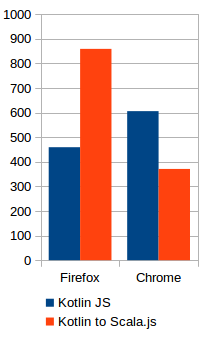
\includegraphics[height=5.5cm]{imgs/deltablue.png}
        \caption{DeltaBlue}
    \end{subfigure}}
    ~
    \onslide<2->{
    \begin{subfigure}[h]{0.30\textwidth}
        \centering
        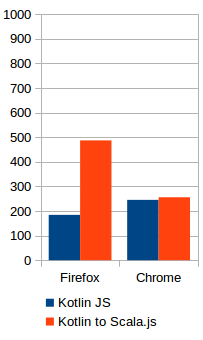
\includegraphics[height=5.5cm]{imgs/richards.png}
        \caption{Richards}
    \end{subfigure}}
    ~
    \onslide<3->{
    \begin{subfigure}[h]{0.30\textwidth}
        \centering
        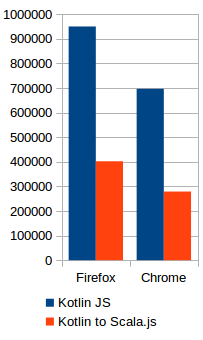
\includegraphics[height=5.5cm]{imgs/sha512.png}
        \caption{SHA512}
    \end{subfigure}}
    \caption*{Results in Firefox and Chrome (execution times, lower is better)}
    \label{chart_chrome}
\end{figure}
\end{frame}


\section{Future work}

\begin{frame}{Future work}
 \begin{itemize}
  \item Suited for small size applications
  \item Regarding performance both compilers have their flaws
  \item Kotlin Standard Library is still not fully compilable
  \item Interactions with HTML DOM are hard, poor dynamic types handling
 \end{itemize}

\end{frame}



\begin{frame}[standout]
  Questions?
\end{frame}

\appendix

\section{Backup slides}


\begin{frame}[fragile]{Type checks and casts}
 \begin{itemize}
  \item Kotlin provides two keywords in order to perform type checking (with \ktinline{is} ) or casts (with \ktinline{as} ) :
 \end{itemize}
 
  \begin{figure}
   \centering
   \begin{subfigure}[h]{0.45\textwidth}
      \begin{minted}[bgcolor=minted-bg]{kotlin}
  myVal is SomeClass
      \end{minted}
      \caption*{Type check}
   \end{subfigure}
   ~
   \begin{subfigure}[h]{0.45\textwidth}
      \begin{minted}[bgcolor=minted-bg]{kotlin}
  myVal as SomeClass
      \end{minted}
      \caption*{Type cast}
   \end{subfigure}

  \end{figure}
  \begin{itemize}
   \item The current version of the compiler doesn't support smart casts.
  \end{itemize}

\end{frame}

\begin{frame}[fragile]{Type checks and casts - a complete example}
 \begin{minted}[bgcolor=minted-bg]{kotlin}
fun casts(anyVal: Any): Unit {
  if (anyVal is Dummy) {
    val d = (anyVal as Dummy)
    // Use d
  } else if (anyVal is Int) {
    val i = anyVal as Int
    // Use i
  } else {
    val s = anyVal.toString()
    // Use s
  }
}
 \end{minted}
\end{frame}

\begin{frame}[fragile]{Type checks and casts - A complete example}
 \begin{minted}[bgcolor=minted-bg]{scala}
static def casts__O__V(anyVal: any) {
  if (anyVal.isInstanceOf[LDummy]) {
    val d: LDummy = anyVal.asInstanceOf[LDummy];
    (void 0)
  } else if (anyVal.isInstanceOf[jl_Integer]) {
    val i: int = anyVal.asInstanceOf[I];
    (void 0)
  } else {
    val s: T = anyVal.toString__T();
    (void 0)
  };
  (void 0)
}
 \end{minted}
\end{frame}

\begin{frame}{Qualified this}
 The keyword \ktinline{this} must be translated in two different ways :
 
 \begin{itemize}
  \item As the SJSIR \scalainline{This()} object
  \item As a reference to the \scalainline{\$this} argument (for extension functions for instance)
 \end{itemize}

\end{frame}


\begin{frame}[fragile]{Enum classes}
 \begin{minted}[bgcolor=minted-bg]{kotlin}
enum class Fruits {
  APPLE, BANANA, PEACH
}
 \end{minted}
 
 \begin{itemize}
  \item Enum entries are classes themselves
  \item The compiler generates the \ktinline{values()} and \ktinline{valueOf(s: String)} methods.
  \item All entries and functions are stored inside a module class
 \end{itemize}
\end{frame}

\begin{frame}[fragile]{Enum classes - A fruity example}
 
  \begin{minted}[bgcolor=minted-bg, breaklines=true]{scala}
// Fruits$APPLE.sjsir, Fruits$BANANA.sjsir and Fruits$PEACH.sjsir
class LFruits$APPLE extends LFruits {
  def init___T__I(_name: T, _ordinal: int) {
    this.LFruits::init___T__I(_name, _ordinal)
  }
}
  \end{minted}
  \begin{minted}[bgcolor=minted-bg, breaklines=true]{scala}
// Fruits.sjsir
class LFruits extends jl_Enum {
  def init___T__I(_name: T, _ordinal: int) {
    this.jl_Enum::init___T__I(_name, _ordinal)
  }
}
  \end{minted}
  
\end{frame}

\begin{frame}[fragile]{Enum classes - Fruits\$.sjsir}
  \begin{minted}[bgcolor=minted-bg, breaklines=true]{scala}
module class LFruits$ extends O {
  def valueOf__T__LFruits(string: T): LFruits = {
    if (string.equals__O__Z("PEACH")) {
      this.PEACH$1    
    } else { /* ... */
      throw new jl_IllegalArgumentException()
        .init___T(/* ... */)
    }
  }
  val $VALUES: LFruits[]
  def values__ALFruits(): LFruits[] = {
    this.$VALUES.clone__O().asInstanceOf[LFruits[]]
  }
  def init___() {
    this.O::init___();
    this.APPLE$1 = new LFruits$APPLE().init___T__I("APPLE", 0);
    // omitting other entries
    this.$VALUES = LFruits[](this.APPLE$1, this.BANANA$1, this.PEACH$1)
  }
}

  \end{minted}
\end{frame}
\begin{frame}{Anonymous objects}
 \begin{itemize}
  \item Translated as normal objects
  \item Declaration is replaced with a \scalainline{New()} SJSIR node
 \end{itemize}

\end{frame}

\begin{frame}[fragile]{Anonymous objects - Example}
 \begin{minted}[bgcolor=minted-bg]{kotlin} 
fun foo() {
  val adHoc = object {
    var x: Int = 0
    var y: Int = 0
  }
  print(adHoc.x + adHoc.y) // prints 0
}
 \end{minted}

  \begin{minted}[bgcolor=minted-bg, breaklines=true]{scala}
def foo__V() {
  val adHoc = new Lfoo_Main$NoNameProvided().init___();
  mod:s_Predef$.print__O__V((adHoc.x__I() +[int] adHoc.y__I()));
  (void 0)
}
  \end{minted}
\end{frame}




\end{document}
